\documentclass[xcolor=table]{beamer}
\usetheme{LSUHSC}
\setbeamertemplate{caption}[numbered]
\usefonttheme[onlymath]{serif}

% ------------------------------------------------------------------------------------------------

\usepackage[utf8]{inputenc}
\usepackage[T1]{fontenc}
\usepackage{helvet}
\usepackage{graphicx} % Allows including images
\usepackage{booktabs} % Allows the use of \toprule, \midrule and \bottomrule in tables
\numberwithin{figure}{section}
\numberwithin{equation}{section}
\usepackage{natbib,verbatim}
\usepackage{multirow}
\usepackage[export]{adjustbox}
\usepackage{todonotes}

% ------------------------------------------------------------------------------------------------

\title[Breast cancer --- Machine learning]{Breast Cancer Type Classification Using Machine Learning Approach}
\author[J. Wu, T. Mamidi, L. Zhang, C. Hicks]{\scriptsize{Jiande Wu, Tarun Mamidi, Lu Zhang, Chindo Hicks}\\{\ttfamily jwu2, tmamid, lzhan1, chick3@lsuhsc.edu}}
\institute{Department of Genetics, LSUHSC\\ Bioinformatics and Genomics (BIG) Program}
\date{\today}

% ------------------------------------------------------------------------------------------------

\begin{document}

% ------------------------------------------------------------------------------------------------

\begin{frame}[plain,t]
\titlepage
\end{frame}

% ------------------------------------------------------------------------------------------------

\begin{frame}%[plain,noframenumbering]
  \addtocounter{framenumber}{-1}
%  \footnotesize
%   \thispagestyle{empty}
  \frametitle{Context}
  \setbeamertemplate{section in toc}[sections numbered]
  \tableofcontents[hideallsubsections]
\end{frame}

% ------------------------------------------------------------------------------------------------

\section{Introduction}
\begin{frame}
 \frametitle{Introduction}
 \begin{itemize}
     \item A common issue in medicine is to distinguish accurately between similar diseases in order to make an accurate diagnosis of a patient. 
     \item Molecular-level classification using gene expression profile has already proven useful for this task.
     \item This tehnique has been used in two tasks: class discovery and class prediction. 
     \begin{itemize}
     \item Class discovery is the task of identifying new classes of cancer.
     \item Class prediction is the task of assigning a new tumor to a known class.
     \end{itemize}
 \end{itemize}
\end{frame}

\begin{frame}
 \frametitle{Introduction}
  \begin{itemize}
    \item Breast cancer is the most diagnosed cancer among women in the US and the second leading cause of cancer-related in women.
    \item Breast cancer is a heterogeneous disease defined by molecular types. 
    \item Accurate prediction of type can aid in effectively directing patient therapy. 
    \item In this study, k-Nearest Neighbours (kNNs), Naive Gaussian Bayes (NGB), Random Tree (RT) and Support Vector Machines (SVM) are proposed to identify two types of breast cancer (Triple Negative and ER positive).
  \end{itemize}
\end{frame}

% ------------------------------------------------------------------------------------------------
\section{Methods}

\begin{frame}{Methods}
%-------------------------------------------------------
\begin{exampleblock}{Given: A set of gene expression data}
\begin{itemize}\footnotesize{
    \item The samples have a group of closely related diseases. 
    \item Each sample gene's numeric expression levels constitute the features of an sample. 
    \item The corresponding disease classification for each sample is that sample's category. }
\end{itemize}
\end{exampleblock}

\begin{exampleblock}{Do: Learn a model that can accurately classify a new sample into its appropriate disease classification}
\begin{itemize}\footnotesize{
    \item We can use any of the supervised learning techniques to induce a diagnosis model from the gene expression data and the associated disease. 
    \item Once an accurate predictive model is obtained, new samples or those who were previously undiagnosable can be classified. }
\end{itemize}
\end{exampleblock}
\end{frame}

\begin{frame}{Methods}{Classification Models}
  \begin{itemize}
      \item We compare the classification performance of a number of important and widely used machine learning algorithms.
      \item  k-Nearest Neighbours (kNNs), Naive Gaussian Bayes (NGB), Random Tree (RT) and Support Vector Machines (SVM).
      \item Using massively parallel processing on high-performance computers, we compare the average accuracy at various combinations of levels of two factors: number of genes, training sample size, 
  \end{itemize}
\end{frame}

\begin{frame}{Methods}{Model Evaluation}
%-------------------------------------------------------
We evaluate and compare of several estimator: 
\begin{itemize}
    \item Hold-out Validation
    \item K-fold Cross Validation (CV)
    \item Bootstrap Resampling
\end{itemize}
\begin{figure}
\centering
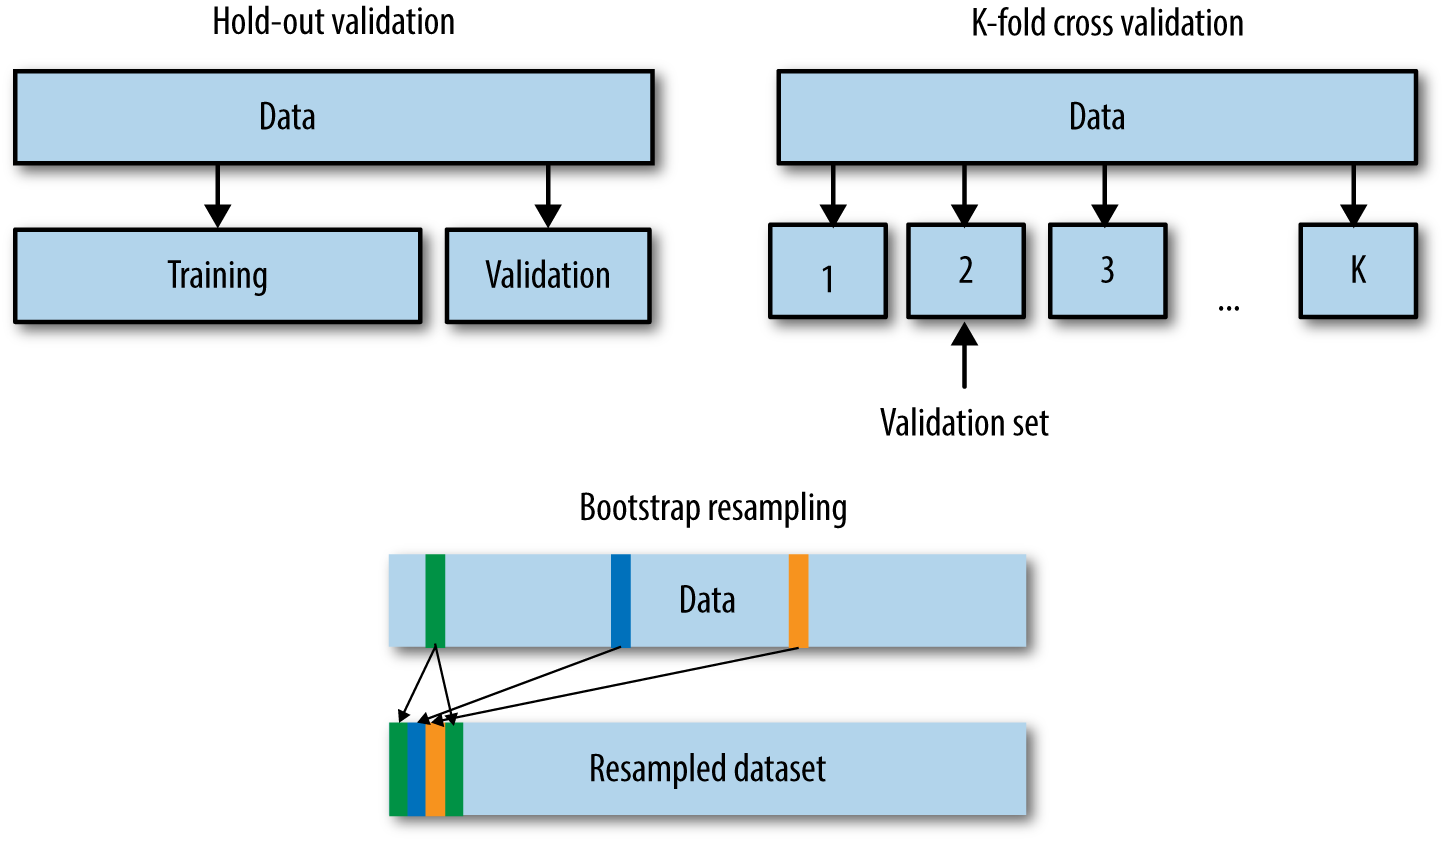
\includegraphics[width=70mm]{pictures/CV.png}
\end{figure}
%https://www.oreilly.com/ideas/evaluating-machine-learning-models/page/4/offline-evaluation-mechanisms-hold-out-validation-cross-validation-and-bootstrapping
%In N-fold cross validation, the examples are divided into N subsets, and then each subset is successively used as the held-aside test set, while the other (N-1) subsets are pooled to create the training set. The results of all N test-set runs are averaged to find the total accuracy. The typical value for N is 10. 
\end{frame}

\begin{frame}{Methods}{Model Evaluation}
%-------------------------------------------------------
\begin{itemize}
    \item  The estimators were compared in terms of bias and variability using simulations for training samples of various sizes. 
    \item We consider training sample sizes (n) ranging from 10 to 210, 
    \item A comparison based on average performance over 10 different training sample sizes shows bootstrap estimators to be less biased, but highly unstable.
    \item Our comparison shows that hold-out estimator has very similar variability to 10-fold CV estimator.
    \item We use 10-fold CV for estimating these performance measures.
\end{itemize}

%In N-fold cross validation, the examples are divided into N subsets, and then each subset is successively used as the held-aside test set, while the other (N-1) subsets are pooled to create the training set. The results of all N test-set runs are averaged to find the total accuracy. The typical value for N is 10. 
\end{frame}

\begin{frame}{Methods}{Performance estimators: Accuracy, Precision, Recall}
%-------------------------------------------------------
We compare performance of the methods in terms of  \textbf{classification accuracy}, \textbf{precision}, and \textbf{recall}.
\begin{table}[]
\begin{tabular}{|c|c|c|}
\hline
                               & \multicolumn{2}{c|}{Predicted Class}                                                      \\ \cline{2-3} 
\multirow{-2}{*}{Actual Class} & \cellcolor[HTML]{CBCEFB}Yes                 & \cellcolor[HTML]{CBCEFB}No                  \\ \hline
\cellcolor[HTML]{CBCEFB}Yes    & \cellcolor[HTML]{32CB00}TP (True Positive)  & \cellcolor[HTML]{FD6864}FN (False Negative) \\ \hline
\cellcolor[HTML]{CBCEFB}No     & \cellcolor[HTML]{FD6864}FP (False Positive) & \cellcolor[HTML]{32CB00}TN (True Negative)  \\ \hline
\end{tabular}
\end{table}
\begin{equation*}
\begin{split}
\textbf{Accuracy:}\qquad A&=\frac{TP+TN}{TP+FP+FN+TN} \\
\textbf{Precision:}\qquad P&=\frac{TP}{TP+FP}\\
\textbf{Recall:}\qquad R&=\frac{TP}{TP+FN}
\end{split}
\end{equation*}
%http://blog.exsilio.com/all/accuracy-precision-recall-f1-score-interpretation-of-performance-measures/
\end{frame}
% ------------------------------------------------------------------------------------------------
\begin{comment}

\subsection{k-Nearest Neighbours (kNNs)}
%-------------------------------------------------------
\begin{frame}{Methods}{k-Nearest Neighbours (kNNs)}
%-------------------------------------------------------
\begin{itemize}
    \item We have an existing set of gene expression data and we know subtypes for all of this data.
    \item When we’re given a new piece of gene expression data without a subtype, we compare that new piece of data to the existing data.
    \item Then take the most similar pieces of data (the nearest neighbors) and look at their subtypes.
    \item Choose the top k most similar pieces of data from our known data set.
    \item Lastly, we take a majority vote from the k most similar pieces of data, and the majority is the new subtype we assign to the data
\end{itemize}

\end{frame}

%-------------------------------------------------------
\subsection{Decision-trees (DTs)}
%-------------------------------------------------------
\begin{frame}{Methods}{Decision-trees (DTs)}
%-------------------------------------------------------
We divide the process into two different steps, the training phase and the prediction phase.
\begin{block}{Training phase}
\begin{itemize}
    \item Make a first decision on the gene data set to dictate which gene is used to split the data.
    \item After that, split the data set into subsets.
    \item If the data on the subsets has the same subtype, then don’t need to continue splitting it.
    \item Otherwise need to repeat the splitting process on this subset.
    \item Repeat this process until classified all the data.
\end{itemize}
\end{block}
\end{frame}
%-------------------------------------------------------
\begin{frame}{Methods}{Decision-tree (DTs)}
%-------------------------------------------------------
\begin{block}{Prediction phase}
\begin{itemize}
    \item Given the gene expression data of a new patient.
    \item At each node in the tree path, only the selected gene for that node in the training phase are tested.
    \item If the patient’s gene profile is classified as a positive sample, then the prediction outcome is the subtype corresponding to that node and the prediction phase terminates.
    \item Otherwise, the sequence of classification tests continues until a leaf is reached, in which case the prediction outcome is the subtype associated with that leaf.
\end{itemize}
\end{block}
\end{frame}

\subsection{Bayesian Method}
\begin{frame}{Methods}{Bayesian Method --- Naive Bayes Classifiers (NBC)}
 \begin{itemize}
     \item NBC models are known under a variety of names, including simple Bayes and independence Bayes.
     \item NBC need strong independence assumptions between the features (genes).
     \item NBC can be trained very efficiently in a supervised learning setting.
     \item An advantage of NBC is that it only requires a small number of training data to estimate the parameters necessary for classification.
     \item Despite their oversimplified assumptions, NBC have worked quite well in many real-world situations.
 \end{itemize}
\end{frame}

\begin{frame}{Methods}{Bayesian Method --- Naive Bayes Classifiers (NBC)}
 \begin{block}{Probabilistic Model}
 \begin{itemize}
     \item  Given a problem instance to be classified, represented by a vector $\mathbf {x} =(x_{1},\dots ,x_{n})$ representing some $n$ features (independent variables), it assigns to this instance probabilities
  \begin{equation*}
   %\label{eqn:definitionDerivative}
   p(C_{k}\mid x_{1},\dots ,x_{n}) \text{ or }  p(C_{k}\mid \mathbf {x})
  \end{equation*}
  for each of $K$ possible classes $C_{k}$.\\
    \item Using Bayes' theorem, the conditional probability can be decomposed as
  \begin{equation*}
   %\label{eqn:definitionDerivative}
   {\displaystyle p(C_{k}\mid \mathbf {x} )={\frac {p(C_{k})\ p(\mathbf {x} \mid C_{k})}{p(\mathbf {x} )}}}
  \end{equation*}
 \end{itemize}
 \end{block}
\end{frame}

% ------------------------------------------------------------------------------------------------
\begin{frame}{Methods}{Bayesian Method --- Naive Bayes Classifiers (NBC)}
 \begin{block}{Cont.}
 \begin{itemize}
     \item  In practice, there is interest only in the numerator, because the denominator does not depend on $C$, so that the denominator is effectively constant.\\
    \item Now using the "naive" conditional independence assumptions
  \begin{equation*}
   %\label{eqn:definitionDerivative}
   {\displaystyle {\begin{aligned}p(C_{k}\mid \mathbf {x})&\varpropto p(C_{k})\ p(\mathbf {x} \mid C_{k})\\&=p(C_{k})\ p(x_{1}\mid C_{k})\ p(x_{2}\mid C_{k})\ \cdots\ p(x_{n}\mid C_{k}) \\&=p(C_{k})\prod _{i=1}^{n}p(x_{i}\mid C_{k})\,.\end{aligned}}}
  \end{equation*}
 \end{itemize}
 \end{block}
\end{frame}
% ------------------------------------------------------------------------------------------------
\begin{frame}{Methods}{Bayesian Method --- Naive Bayes Classifiers (NBC)}
 \begin{block}{Naive Bayes Classifiers}
   \begin{itemize}
    \item The NBC combines this probabilistic model with a decision rule. One common rule is to pick the hypothesis that is most probable.
    \item A class's prior $p(C_{k})$ may be calculated by using prior statistic information, or by calculating an estimate for the class probability from the training set.
    \item The assumptions on distributions of features $p(x_{i}\mid C_{k})$.
     \begin{itemize}
         \item Multinomial Bayes
         \item Gaussian Bayes
         \item Bernoulli Bayes
     \end{itemize}
  \end{itemize}
 \end{block}
\end{frame}

% ------------------------------------------------------------------------------------------------
\begin{frame}{Methods}{Bayesian Method --- Naive Bayes Classifiers (NBC)}
 \begin{block}{Determine which posterior is greater, TNBC or ER+}
 \footnotesize{
   \begin{itemize}
    \item Assume that we have a dataset with two classes $(\text{TNBC},\text{ER+})$.
    \item For the classification as TNBC the posterior is given by
  \begin{equation*}
   %\label{eqn:definitionDerivative}
   \scriptsize{
   {\displaystyle {\text{posterior (TNBC)}}={\frac {p({\text{TNBC}})\,p({\text{gene}_1}\mid {\text{TNBC}})\dots\,p({\text{gene}_n}\mid {\text{TNBC}})}{evidence}}}}
  \end{equation*}
    \item For the classification as $\text{ER+}$ the posterior is given by
  \begin{equation*}
   %\label{eqn:definitionDerivative}
   \scriptsize{
   {\displaystyle {\text{posterior (ER+)}}={\frac {p({\text{ER+}})\,p({\text{gene}_1}\mid {\text{ER+}})\dots\,p({\text{gene}_n}\mid {\text{ER+}})}{evidence}}}}
  \end{equation*}
   \item The $evidence$ is a constant. It therefore does not affect classification and can be ignored.
   \item To classify a new sample with genes $\mathbf {g} = (g_1,\dots, g_n)$, we use the following rules:
     \begin{itemize}
         \item If $p(\text{TNBC} \mid \mathbf {g}) >p(\text{ER+} \mid \mathbf {g})$, then the class is $\text{TNBC}$.
         \item If $p(\text{TNBC} \mid \mathbf {g}) <p(\text{ER+} \mid \mathbf {g})$, then the class is $\text{ER+}$.
     \end{itemize}
  \end{itemize}}
 \end{block}
\end{frame}

\subsection{Logistic Regression}
\begin{frame}{Methods}{Logistic Regression (LG)}
    Pros:
    \begin{itemize}
        \item Computationally inexpensive
        \item Easy to implement
        \item Knowledge representation easy to interpret 
    \end{itemize}
    Cons:
    \begin{itemize}
        \item Prone to underfitting
        \item May have low accuracy
    \end{itemize}
    Works with: Numeric values, nominal values
\end{frame}
\end{comment}
% ------------------------------------------------------------------------------------------------
\section{Data Set}
%-------------------------------------------------------

\begin{frame}{Data Set}
  \begin{itemize}
      \item This dataset is based on a gene expression study of breast cancer from TCGA. 
      \item Gene expression data was merged with clinical information to ascertain the disease type. 
      \item The data matrix was filtered to remove rows with missing data, such that each row has at least $\geq 30\%$ data.
      %\item We use clinical information to classify samples into two groups: triple negative breast cancer patients, and normal.
      \item To begin, we select those 200 genes from the 45,000 genes on the gene expression data with the highest degree of association with the disease outcome. (Calculated by gene different expression p-value over the full set of 210 samples, we then rank these genes by their p-value.) %They repeat "leave-one-out" cross-validation over all 78 examples using various ensemble sizes. We found that an ensemble size of 70 genes gives the best cross-validated accuracy (83\%). 
  \end{itemize}
 
\end{frame}

\section{Results \& Discussions}
%-------------------------------------------------------
\begin{comment}
\subsection{k-Nearest Neighbours (kNNs)}
\subsection{Decision-trees (DTs)}
\subsection{Bayesian Method}
\begin{frame}{Results \& Discussions}{Bayesian Method --- Naive Bayes Classifiers (NBC)}
%-------------------------------------------------------
 \begin{itemize}
     \item Despite the fact that the independence assumptions are often inaccurate, the NBC has several properties that make it useful in practice.
     \begin{itemize}
         \item Each feature distribution can be independently estimated as a one-dimensional distribution.
         \item Works with a small amount of data, handles multiple classes.
     \end{itemize}
 \begin{alertblock}{???}
  \footnotesize{Our results support that the proposed approach to gene selection yields a small subset of genes that can predict these two breast cancer types with greater than 95\% overall accuracy.}
 \end{alertblock}
    \item It is very much sensitive to outliers. It is one of the most important drawbacks for gene expression data analysis by the NBC. The gene expression dataset is often contaminated by outliers.
 \end{itemize}
\end{frame}
\end{comment}

\begin{frame}{Results \& Discussions}{Average accuracy at varying levels of training sample and feature sizes}
\begin{figure}
\begin{subfigure}
  \centering
  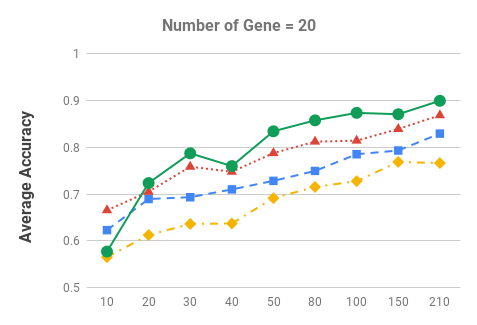
\includegraphics[scale=0.18,valign=t]{pictures/NumberofGene=20.png}
\end{subfigure}
\begin{subfigure}
  \centering
  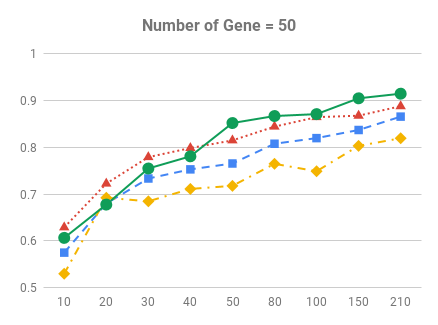
\includegraphics[scale=0.18,valign=t]{pictures/NumberofGene=50.png}
\end{subfigure}
\begin{subfigure}
  \centering
  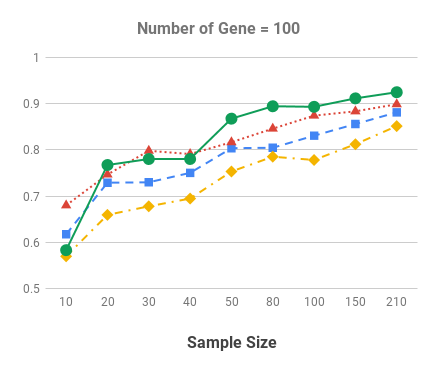
\includegraphics[scale=0.18,valign=t]{pictures/NumberofGene=100.png}
\end{subfigure}
\hspace{-.9in}\begin{subfigure}
  \centering
  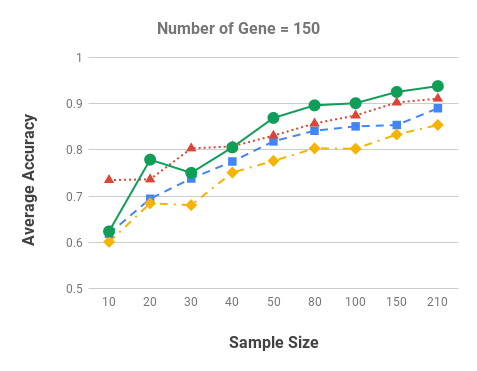
\includegraphics[scale=0.18]{pictures/NumberofGene=150.png}
\end{subfigure}
\begin{subfigure}
  \centering
  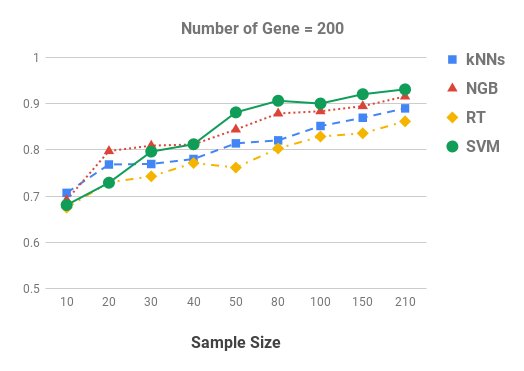
\includegraphics[scale=0.18]{pictures/NumberofGene=200.png}
\end{subfigure}
  \textcolor{white}{\rule{2.4cm}{2cm}}
\end{figure}
\begin{itemize}
    \item \footnotesize{Although the performance of SVM was found to be better than the other methods for larger training samples and feature sets, the method does not perform well for smaller ($n \le 40$) samples.}
\end{itemize}
\end{frame}

\begin{frame}{Results \& Discussions}{Average accuracy at varying levels of training sample and feature sizes}
\begin{figure}
\begin{subfigure}
  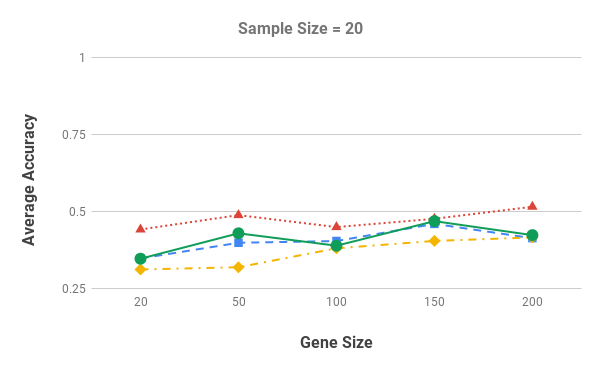
\includegraphics[scale=0.14]{pictures/SampleSize=20.png}
\end{subfigure}
\begin{subfigure}
  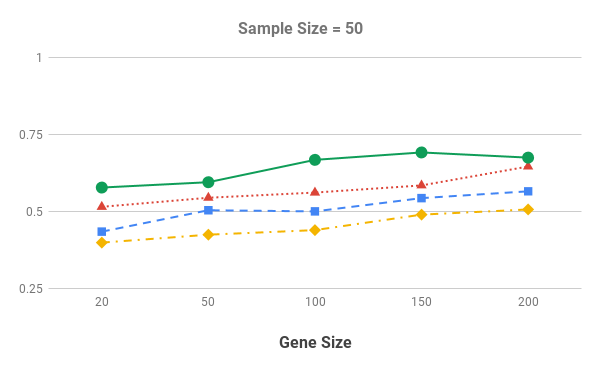
\includegraphics[scale=0.14]{pictures/SampleSize=50.png}
\end{subfigure}
\begin{subfigure}
  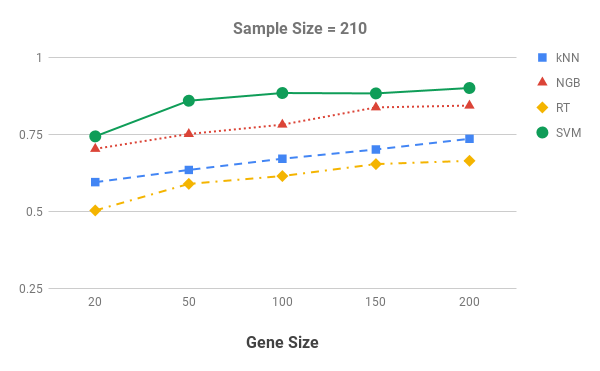
\includegraphics[scale=0.14]{pictures/SampleSize=210.png}
\end{subfigure}
\end{figure}    
\begin{itemize}
    \item \footnotesize{Although their performance is improved when the number of genes is increased, the performance is not improved much when the number of genes exceeds 150.}
\end{itemize}
\end{frame}
%-------------------------------------------------------
\section{Conclusions \& Future work}
%-------------------------------------------------------
\begin{frame}[allowframebreaks]{Conclusions}
  \begin{itemize}
    \item As the feature set gets larger SVM performs better than kNNs, NGB and RT.
    \item The performance of NGB also increases as the feature set size increases, and exceeds the performance of kNN and RT unless the amount of data is too small.
    \item RT was found to outperform only NGB in some instances where the data had smaller effect sizes, in which cases it also provided more stable error estimates than NGB.
    \item The performance is improved when feature set size is increased, But the performance improvement is not very good when the number of genes exceeds 150.
  \end{itemize}
\framebreak
  The main contributions of this work:
\begin{itemize}
    \item We performed an extensive study in order to objectively compare classification performance of a number of widely used machine learning in terms of accuracy.
    \item k-Nearest Neighbours (kNNs), Naive Gaussian Bayes (NGB), Random Tree (RT) and Support Vector Machines (SVM) are implemented.
  \item None of the methods studied (except NGB) require data to follow any particular probability distribution, and the simulation results should be able to resist deviations from the normal hypothesis.
\end{itemize}
\framebreak
  \begin{itemize}
    \item The main focus of our study was to investigate ``which method performs better in what circumstances'' by comparing performance at various combinations of levels of multiple factors.
    \item A new method for predicting gene selection for breast cancer types was proposed.
      \item We have discovered a new set of compact genes that can be used to differentiate between breast cancer and normal in a clinical setting.
 \end{itemize}
 \end{frame}

\begin{frame}[allowframebreaks]{Discussion \& Future work}
    \begin{itemize}
        \item I realized that the characteristics and relative performance of each algorithm can vary depending on the details of the data (and the degree of adjustment).
        \item Trying to build an "objective" comparison is an unwise task.
        \item It is still valuable to provide this result as a set of general guidelines and as a starting point for algorithms that compare future genetic research tasks.
    \end{itemize}
\framebreak
    This achievement is the result of my own experience. Please tell me how you can improve this work.
\begin{itemize}
    \item Are there other "important" criteria for comparison that should be added to this work?
    \item Are there any other algorithms that you would like me to add to this work? 
\end{itemize}
\end{frame}
% ------------------------------------------------------------------------------------------------

\ThankYouFrame

% ------------------------------------------------------------------------------------------------

\end{document}
